\chapter{FAHP多维资源建模和参数自动求解}
在上一节新的评分函数中,根据资源的重要程度使用\begin{math}\alpha_{i}(i=1,2,3,4,5),  alpha_{1}+\alpha_{2}+\alpha_{3}+\alpha_{4}+\alpha_{5}=1\end{math}作为CPU、内存、磁盘I/O、网络带宽和已部署Pod数量的重要程度系数。本章需要对预选筛选后的节点资源进行建模,并利用FAHP方法进行调度Pod多维权重参数的自动求解。

\section{模糊层次分析法FAHP}
模糊层次分析法FAHP(Fuzzy Analytical Hierarchy Process)是在层次分析法的基础发展而来,常用于解决实际问题中影响决策问题的多种因素的权重。下面从层次分析法开始介绍,为弥补层次分析法的不足引入FAHP方法,然后举例说明如何使用该方法解决实际问题。

\subsection{FAHP方法介绍}
在面对许多实际问题解决方案时,我们往往需要对影响方案的因素进行比较、判断、评价,然后做出决策,这种人工主观解决问题的方式不但效率低下,结果也不够准确。层析分析法(Analytical Hierarchy Process)是由著名的美国运筹学家匹茨堡大学T.L.Saaty教授提出的一种层次权重决策分析方法。该方法用于解决复杂的多目标决策问题,将影响目标决策的因素分解为目标层、准则层和方案层等层次,使用数学方法对个因素进行精确求解。层次分析法将问题的总目标、各层子目标以及决策因素分解成多个层次结构,然后构建各层次的判断矩阵,求解判断矩阵的特征值。最大特征值对应的特征向量归一化获得本层各元素上一层次某元素的优先权重,最后再加权和的方法递阶归并各备择方案对总目标的最终权重,选择最终权重最大的方案作为选择的方案。该方法是一个系统性的分析方法,先将问题分解成多个层次,然后对影响子目标的因素进行比较判断、最终进行综合决策。结构层次清晰、单层的权重参数设置都会影响到最终的决策层,不断分割量化各因素的影响。层次分析法非常实用,将定量分析和定性分析相结合,解决许多实际问题如电力分配、旅游决策等,该方法计算简单明了,易于掌握。最后,该方法具有简洁性,用于模拟人们解决问题的思维,所需的定量信息较少,仅需要对影响决策因素的重要性做出判断即可。

但是,层次分析法也具有局限性,在一些场景下无法使用或者效果较差。首先,该方法只能从实际的备选方案中帮助决策者选出较优的决策方案,不能给决策者提供新的解决方案或者反馈合理方案的意见,此外,该方法是单目标决策方法,使用者只能选出一个最优的目标。其次,该方法模拟人类大脑决策过程,定性分析过于浓厚,只能进行粗略比较计算,不能完全做到精确模拟。最后,从层次结构转化为成对比矩阵过程中,判断者的主观因素影响过大,判断者不同,得出的最优方案也不尽相同,无法让人信服。并且随着影响决策因素的增加,构建的成对比矩阵阶数增大,计算难度和复杂度随之增加,很难一次性构建出满足一致性要求的成对比矩阵。

为减少人为主观因素对决策结果的影响,模糊层析分析法FAHP在层次分析法的基础上增加人为判断的模糊性,具体而言就是层析分析通过两两比较构建成对比判断矩阵,FAHP通过两两比较构建模糊成对比矩阵,提升了层次分析法解决问题的可靠性。在进行问题判断或专家咨询时,往往不是给出一个具体值,而是一个模糊数,如三值判断(最低可能值、最可能值和最大可能值)、二值区间等。下面先介绍模糊数集的概念,对于一个明确的集合:
\begin{equation}
\mu_{A}(x) = \left\{\begin{array}{l}
1, x\in A \\ [0.3cm]
0, x\notin A
\end{array}\right.
\end{equation}
明确的集合中,\begin{math}x\in A\end{math}时值为1,\begin{math}x\notin A\end{math}时值为0.但对于一个模糊数集,并不能完全明确x是否属于A,只能用[0,1]表示其隶属度。
\begin{equation}
\mu_{A}(x):U\to[0,1]
\end{equation}
\begin{math}\mu_{A}(x)\end{math}表示\begin{math}x\in A\end{math}的隶属度,也称\begin{math}\mu_{A}(x)\end{math}为集合A的隶属函数。对于任意的模糊数集,都对应一个隶属函数,隶属函数通常模仿概率论中的分布函数如正态分布、梯形分布、K次抛物线分布、S分布以及柯西分布等,值域在[0,1]上。

1983年,荷兰学者Van Loargoven首次提出用三角模糊数作为模糊数集的判断标准,并运用三角模糊数的运算和对数最小二乘法获取权重值。设论域R上的模糊数M为三角模糊数,M对应的隶属函数\begin{math}\mu_{M:}R\to[0,1]\end{math}满足下列函数:
\begin{equation}
\mu_{M}(x) = \left\{\begin{array}{l}
0 \quad x<a \\ [0.3cm]
\frac{x-a}{b-a} \quad a\le x\le b \\ [0.2cm]
\frac{c-x}{c-b} \quad b\le x\le c \\ [0.2cm]
0 \quad x>c
\end{array}\right.
\end{equation}
M=(a,b,c)其中\begin{math}a\le b\le c\end{math},
a和c分别表示三角模糊数的上界和下界值,b是隶属度为1的中间值,x=b时表示x完全属于M,在a和c之外的完全不属于模糊数M。定义一个置信度\begin{math}\alpha\end{math}可以将三元组的模糊数M化为一个\begin{math}\alpha\end{math}割集的二元形式,从而构建割集矩阵,设定优化参数后将二元值的矩阵转化成最终的判断矩阵。
\begin{equation}
	M_{\alpha} = [l^{\alpha},u^{\alpha}]=[(b-a)\alpha+a,-(c-b)\alpha+c] \quad \forall \alpha\in[0,1]
\end{equation}
根据Arnold J. Kaufmann在文献[xx]中的描述,\begin{math}\alpha\end{math}割集后的基本运算规则如下:
\begin{equation}
\begin{split}
	M_{\alpha} &= [m_{L}^{\alpha},m_{R}^{\alpha}] \\[0.2cm]
	N_{\alpha} &= [n_{L}^{\alpha},n_{R}^{\alpha}] \\[0.2cm]
	M_{\alpha}\oplus N_{\alpha} &= [m_{L}^{\alpha}+n_{L}^{\alpha},m_{R}^{\alpha}+n_{R}^{\alpha}] \\[0.2cm]
	M_{\alpha}\ominus N_{\alpha} &= [m_{L}^{\alpha}-n_{L}^{\alpha},m_{R}^{\alpha}-n_{R}^{\alpha}] \\[0.2cm]
	M_{\alpha}\otimes N_{\alpha} &= [m_{L}^{\alpha}n_{L}^{\alpha},m_{R}^{\alpha}n_{R}^{\alpha}] \\[0.2cm]
	M_{\alpha}\oslash N_{\alpha} &= [m_{L}^{\alpha}/n_{L}^{\alpha},m_{R}^{\alpha}/n_{R}^{\alpha}] \\[0.2cm]
	\end{split}
\end{equation}
本文采用三角模糊数进行FAHP的权重参数求解,并将三元组的M=(a,b,c)转化成\begin{math}\alpha\end{math}割集形式
\begin{math}M_{\alpha} =[(b-a)\alpha+a,-(c-b)\alpha+c] \quad \forall \alpha\in[0,1]\end{math}。

\subsection{FAHP求解权重参数步骤}
介绍完层次分析方法和模糊层析分析方法以及模糊数的基本概念后,下面用三角模糊数作为模糊程度的衡量值,FAHP求解权重参数步骤如下:
\begin{figure}[H] % use float package if you want it here
	\centering
	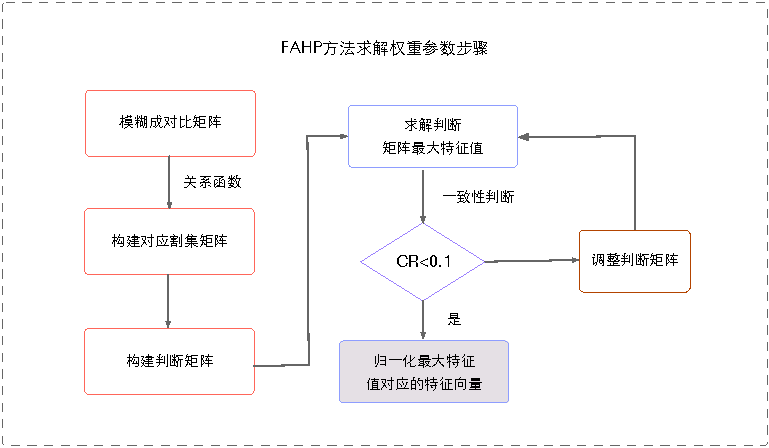
\includegraphics{fahp-flow}
	\caption{FAHP计算权重参数过程}
	\label{fig:xfig1}
\end{figure}
如图4.2所示,使用FAHP方法计算权重参数的步骤可以分为构建模糊成对比矩阵、转化为二元割集矩阵、设置优化参数转化为判断矩阵,求解判断矩阵的最大特征值,检验特征值满足一致性要求,若满足则将最大特征值对应的特征向量归一化作为权重参数值,否则需要调整判断矩阵值,重新进行特征值计算。下面详细介绍求解步骤:

1) 构建模糊成对比矩阵。在FAHP中,对影响决策因素进行两两对比时使用\begin{math}\widetilde{1}\sim \widetilde{9}\end{math}表示其相对重要程度,值越大,表示该因素相对另一个因素对决策目标的影响越大,重要性越高。模糊数、相对重要程度、M三元组及其\begin{math}\alpha \end{math}割集如表4.1所示,可以构建最终的模糊成对比矩阵\begin{math}\widetilde{A} \end{math},其中的元素\begin{math}\widetilde{a_{ij}} \end{math}表示因素i相对j的重要程度,模糊成对比矩阵中元素素值如式(4-6)所示。
\begin{equation}
\widetilde{a_{id}} = \left\{\begin{array}{l}
1 \quad i=i \\ [0.2cm]
\widetilde{1},\widetilde{3},\widetilde{5},\widetilde{7},\widetilde{9}\ or\ \widetilde{1}^{-1},\widetilde{3}^{-1},\widetilde{5}^{-1},\widetilde{7}^{-1},\widetilde{9}^{-1} \quad i\not=j  
\end{array}\right.
\end{equation}
\begin{table}[htbp]
	\centering\dawu[1.3]
	\caption{模糊数、相对重要程度和割集关系表}
	\begin{tabular}{|c|c|c|c|c|c|} \hline
		模糊数 & $\widetilde{1}$ & $\widetilde{3}$ & $\widetilde{5}$  & $\widetilde{7}$ & $\widetilde{9}$ \\ \hline
		重要性 & 同等重要 & 稍微重要 & 重要 & 明显重要 & 非常重要 \\ \hline 
		$\widetilde{M}$ & (1,1,3) & (1,3,5) & (3,5,7) & (5,7,9) & (7,9,11) \\ \hline 
		$\widetilde{M}_{\alpha}$ & [1,3-2$\alpha$] & [1+2$\alpha$,5-2$\alpha$] & [3+2$\alpha$,7-2$\alpha$] & [5+2$\alpha$,9-2$\alpha$] & [7+2$\alpha$,11-2$\alpha$]\\ \hline 
	\end{tabular}
\end{table}

2) 构建割集矩阵并转化为判断矩阵。构建模糊成对比矩阵后,根据表4.1将模糊数转化成三元组的三角模糊数,给定$\alpha$后,将三元组转化成$\alpha$割集\begin{math}\widetilde{M}_{\alpha}=[l_{\alpha},u_{\alpha}]\end{math},从而构建一个$\alpha$割集矩阵$\widetilde{A}_{\alpha}$,割集矩阵中的元素$\widetilde{a}_{ij}^{\alpha}$如式(4-7)所示。给定一个优化参数表示判断优化程度,可以将二元组的割集矩阵转化成判断矩阵A,从而可以对判断矩阵进行特征值和特征向量的求解。设给定的优化参数$\mu\in[0,1]$,用割集矩阵中上下界转化成判断矩阵的单值,判断矩阵中的元素$a_{ij}=(1-\mu)l_{\alpha}+\mu u_{\alpha}$,如式(4-8)所示。通过给定$\alpha$获得二元组的割集矩阵,给定割集矩阵一个优化参数$\mu$可以得到最终的判断矩阵A。
\begin{equation}
\widetilde{a}_{ij}^{\alpha} = \left\{\begin{array}{l}
1 \quad \widetilde{a}_{ij}=1 \\ [0.2cm]
[l_{\alpha},u_{\alpha}] \quad \widetilde{a}_{ij}\in{\widetilde{1},\widetilde{3},\widetilde{5},\widetilde{7},\widetilde{9}} \\ [0.2cm]
[\frac{1}{u_{\alpha}},\frac{1}{l_{\alpha}}] \quad \widetilde{a}_{ij}\in{\widetilde{1}^{-1},\widetilde{3}^{-1},\widetilde{5}^{-1},\widetilde{7}^{-1},\widetilde{9}^{-1}}
\end{array}\right.
\end{equation}
\begin{equation}
a_{ij} = \left\{\begin{array}{l}
1 \quad \widetilde{a}_{ij}=1 \\ [0.2cm]
(1-\mu)l_{\alpha}+\mu u_{\alpha} \quad \widetilde{a}_{ij}\in{\widetilde{1},\widetilde{3},\widetilde{5},\widetilde{7},\widetilde{9}} \\ [0.2cm]
\frac{1-\mu}{u_{\alpha}}+\frac{\mu}{l_{\alpha}} \quad \widetilde{a}_{ij}\in{\widetilde{1}^{-1},\widetilde{3}^{-1},\widetilde{5}^{-1},\widetilde{7}^{-1},\widetilde{9}^{-1}}
\end{array}\right.
\end{equation}

3) 计算判断矩阵最大特征值和特征向量。对判断矩阵特征值的求解是一个纯数学问题,通常用于求解方阵特征值和特征向量的方法有几何平均法(方根法)、算术平均平均法(和法)、最小二乘法(幂法)和特征向量法。通常几种方式求解的特征值很相近,但也存在细微的差别,这些小的差别对实际生产会造成一定的影响。通常而言,几何平均法和算术平均获得的结果精确度较差,最小二乘法计算复杂度较高,因此使用特征向量法对判断矩阵的特征值和特征向量进行求解。在本文中,直接使用Python中numpy库eig()函数求解判断矩阵的特征值和特征向量。

4) 一致性检验和归一化权重。通过特征向量法获得判断矩阵的最大特征值$\lambda_{max}$及其对应的特征向量$\nu_{max}$后,需要进行层次但排序和层次总排序的一致性检验,用于反映特征向量和真实权值的契合度,即检测权重值是否合理。判断矩阵一致性检测方法公式如式(4-9)所示。
\begin{equation}
\begin{split}
CI &= \frac{\lambda_{max}-n}{n-1} \\
CR &= \frac{CI}{RI}
\end{split}
\end{equation}
其中,$\lambda_{max}$是判断矩阵最大特征值,n是影响决策因素的数量即判断矩阵的阶数,CI表示一般一致性指标,RI是随机一致性指标,因此CR是随机一致性比率。若CR<0.1则判断矩阵满足一致性要求,否则需要调整判断矩阵直至其满足一致性判断要求。当CR<0.1时将$\lambda_{max}$对应的特征向量$\nu_{max}$归一化,其值w就是所需求解的权重值。常用的随机一致性指标RI的值如表4.2所示。
\begin{table}[htbp]
	\caption{随机一致性指标RI值}
	\begin{center}
	\begin{tabular}{|p{0.8cm}<{\centering}|p{0.8cm}<{\centering}|p{0.8cm}<{\centering}|p{0.8cm}<{\centering}|p{0.8cm}<{\centering}|p{0.8cm}<{\centering}|p{0.8cm}<{\centering}|p{0.8cm}<{\centering}|p{0.8cm}<{\centering}|p{0.8cm}<{\centering}|p{0.8cm}<{\centering}|} \hline
	n & 1 & 2 & 3 & 4 & 5 & 6 & 7 & 8 & 9 & 10 \\ \hline
	RI & 0 & 0 & 0.58 & 0.90 & 1.12 & 1.24 & 1.32 & 1.41 & 1.45 & 1.49 \\ \hline
	\end{tabular}
\end{center}
\end{table}

以上是用FAHP方法求解权重参数的全部过程,首先对影响决策的因素进行两两比较,构建模糊成对比矩阵,用$\widetilde{1}\sim \widetilde{9}$表示相对重要程度。根据成对比矩阵,给定$\alpha\in[0,1]$获得割集矩阵,设定优化参数$\mu \in[0,1]$获得判断矩阵,计算判断矩阵的最大特征值和对应的特征向量,检测最大特质值是否满足一致性要求,最后将最大特征向量归一化获得权重值。

\subsection{FAHP求解权重参数示例}
上述介绍了FAHP求解权重参数的详细流程和计算方法,下面通过一个简单的例子展示该方法求解权重参数的计算过程,假设在一个物理问题中力学指数的评价由巴氏硬度、耐荷重性、耐冲击性和满水变形四个因素决定,其影响力学指数的判断因素如图4.2所示。
\begin{figure}[H] % use float package if you want it here
	\centering
	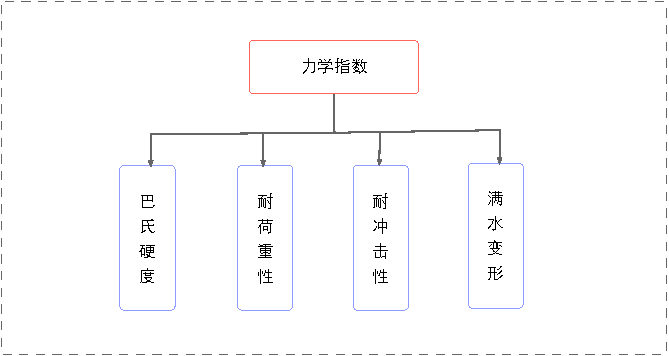
\includegraphics{fahp-example}
	\caption{力学指数的评价因素}
	\label{fig:xfig1}
\end{figure}
某专家通过对影响力学指数的因素进行两两对比后给出其三角模糊判断数,根据其给出的模糊数构建模糊成对比矩阵式(4-10),从左至右一次为巴氏硬度、耐荷重性、耐冲击性和满水变形。
\begin{equation}
\widetilde{A} = \left\{\begin{array}{l}
1 \quad \widetilde{3} \quad \widetilde{7} \quad \widetilde{5}  \\
\widetilde{3}^{-1} \quad 1 \quad \widetilde{5} \quad \widetilde{3} \\
\widetilde{7}^{-1} \quad \widetilde{5}^{-1} 1 \quad \widetilde{3}^{-1} \\
\widetilde{5}^{-1} \quad \widetilde{3}^{-1} \quad \widetilde{3} \quad 1 \\
\end{array}\right\}
\end{equation}
给定$\alpha=0.5$和优化参数$\mu=0.5$,根据式(4-7)和(4-8)可以获得割集矩阵和判断矩阵,判断矩阵A如下:
\begin{equation}
A = \left\{\begin{array}{l}
1 \quad 3 \quad 7 \quad 5 \\
\frac{3}{8} \quad 1 \quad 5 \quad 3 \\
\frac{7}{48} \quad \frac{5}{24} \quad 1 \quad \frac{3}{8} \\
\frac{5}{24} \quad \frac{3}{8} \quad 3 \quad 1 \\
\end{array}\right\}
\end{equation}

使用特征向量法对判断矩阵进行特征值和特征向量求解,最大特征值$\lambda_{max}=4.21154$,其对应的特征向量值$\nu_{max}=[0.88297,0.41986,0.08951,0.18992]$,使用最大特征值对帕判断矩阵A的一致性进行判断,CR=0.082<0.1满足一致性要求。对其最大特征值对应的特征向量进行归一化,其权重w=[0.558,0.265,0.057,0.120]分别表示巴氏硬度、耐荷重性、耐冲击性和满水变形四个因素对力学系数影响的权重系数,用于对后面的目标层做出决策。















